\documentclass[11pt]{article}
\usepackage[textwidth=18.0cm, textheight=23.0cm, top=2.0cm]{geometry}
\usepackage{pst-all}
\usepackage{amssymb}
\usepackage{tikz}
\usepackage{underscore}\begin{document}
\pagestyle{empty}


ClassName: \underline{\textbf{Class_07.2bp-21}}
\par
BinSize: \underline{\textbf{100 × 100}}
\par
ReduceSize: \underline{\textbf{100 × 100}}
\par
TypeNum: \underline{\textbf{59}}
\par
Num: \underline{\textbf{60}}
\par
OutS: \underline{\textbf{140000}}
\par
InS: \underline{\textbf{123761}}
\par
Rate: \underline{\textbf{0.884}}
\par
UB: \underline{\textbf{14}}
\par
LB0: \underline{\textbf{14}}
\par
LB: \underline{\textbf{14}}
\par
LBWithCut: \underline{\textbf{14}}
\par
NodeCut: \underline{\textbf{0}}
\par
ExtendedNodeCnt: \underline{\textbf{1}}
\par
GenNodeCnt: \underline{\textbf{1}}
\par
PrimalNode: \underline{\textbf{0}}
\par
ColumnCount: \underline{\textbf{14}}
\par
TotalCutCount: \underline{\textbf{0}}
\par
RootCutCount: \underline{\textbf{0}}
\par
LPSolverCnt: \underline{\textbf{1}}
\par
PricingSolverCnt: \underline{\textbf{0}}
\par
BranchAndBoundNum: \underline{\textbf{1}}
\par
isOpt: \underline{\textbf{true}}
\par
TimeOnInitSolution: \underline{\textbf{0.140 s}}
\par
TimeOnPrimal: \underline{\textbf{0.000 s}}
\par
TimeOnPricing: \underline{\textbf{0.000 s}}
\par
TimeOnRmp: \underline{\textbf{0.078 s}}
\par
TotalTime: \underline{\textbf{0.280 s}}
\par
\newpage


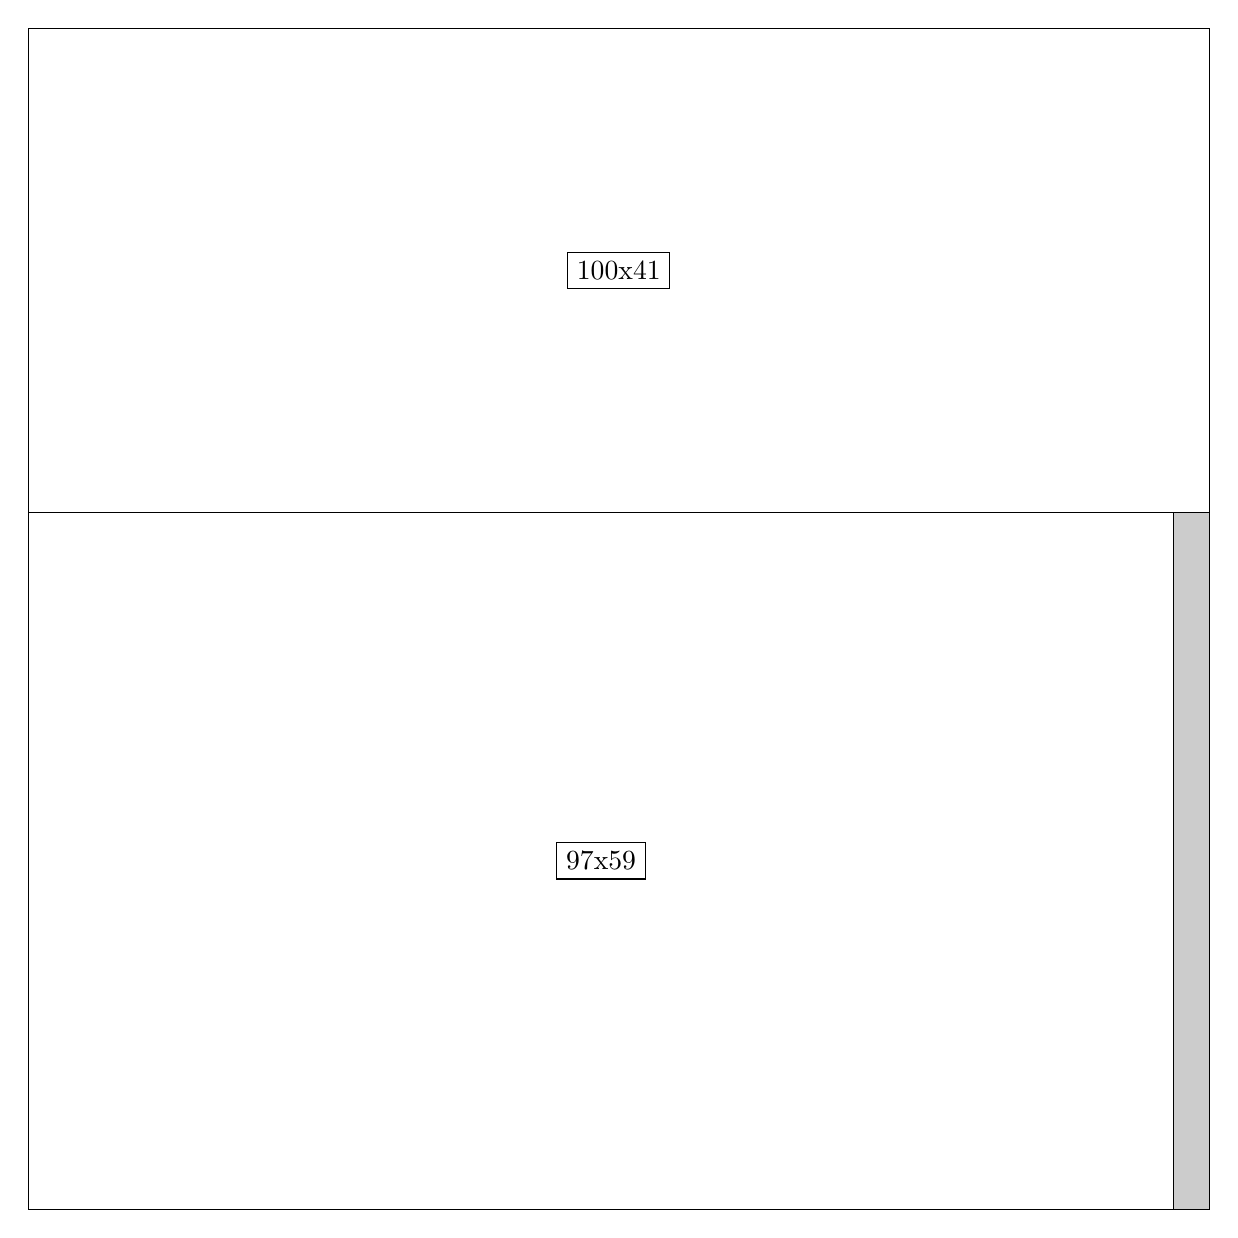
\begin{tikzpicture}[shorten >=1pt,scale=1.0,every node/.style={scale=1.0},->]
\tikzstyle{vertex}=[circle,fill=black!25,minimum size=14pt,inner sep=0pt]
\filldraw[fill=gray!40!white, draw=black] (0,0) rectangle (15.0,15.0);
\foreach \name/\x/\y/\w/\h in {97x59/0.0/0.0/14.549999999999999/8.85,100x41/0.0/8.85/15.0/6.1499999999999995}
\filldraw[fill=white!40!white, draw=black] (\x,\y) rectangle node[draw] (\name) {\name} ++(\w,\h);
\end{tikzpicture}


w =97 , h =59 , x =0 , y =0 , v =5723
\par
w =100 , h =41 , x =0 , y =59 , v =4100
\par
\newpage


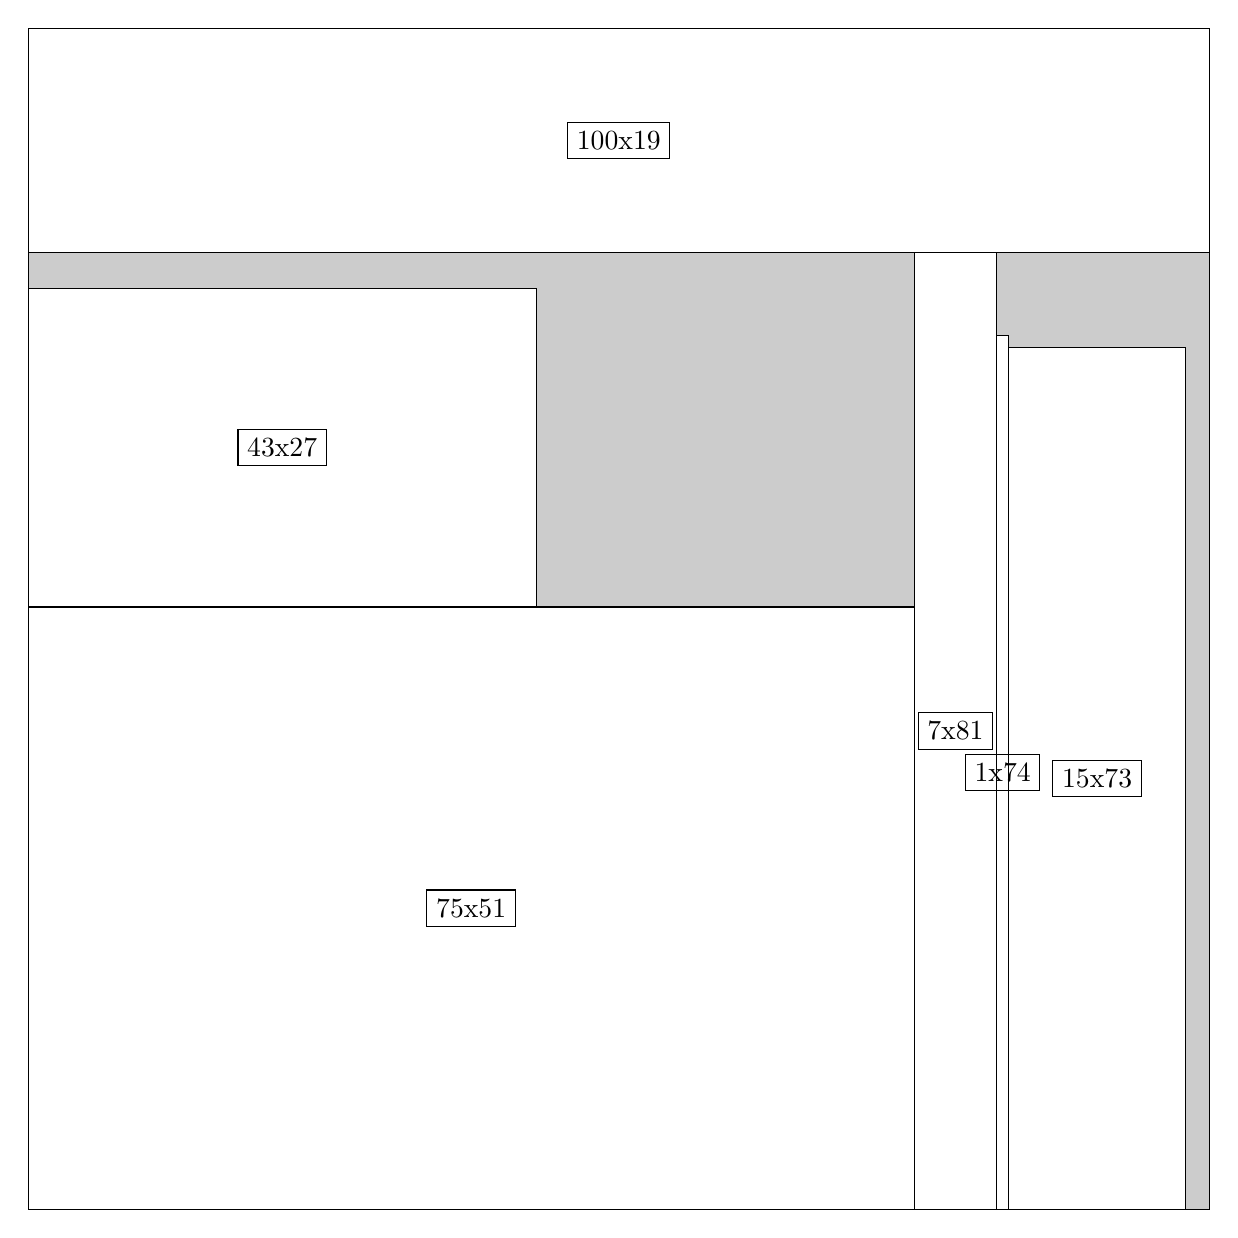
\begin{tikzpicture}[shorten >=1pt,scale=1.0,every node/.style={scale=1.0},->]
\tikzstyle{vertex}=[circle,fill=black!25,minimum size=14pt,inner sep=0pt]
\filldraw[fill=gray!40!white, draw=black] (0,0) rectangle (15.0,15.0);
\foreach \name/\x/\y/\w/\h in {75x51/0.0/0.0/11.25/7.6499999999999995,100x19/0.0/12.15/15.0/2.85,43x27/0.0/7.6499999999999995/6.45/4.05,15x73/12.45/0.0/2.25/10.95,7x81/11.25/0.0/1.05/12.15,1x74/12.299999999999999/0.0/0.15/11.1}
\filldraw[fill=white!40!white, draw=black] (\x,\y) rectangle node[draw] (\name) {\name} ++(\w,\h);
\end{tikzpicture}


w =75 , h =51 , x =0 , y =0 , v =3825
\par
w =100 , h =19 , x =0 , y =81 , v =1900
\par
w =43 , h =27 , x =0 , y =51 , v =1161
\par
w =15 , h =73 , x =83 , y =0 , v =1095
\par
w =7 , h =81 , x =75 , y =0 , v =567
\par
w =1 , h =74 , x =82 , y =0 , v =74
\par
\newpage


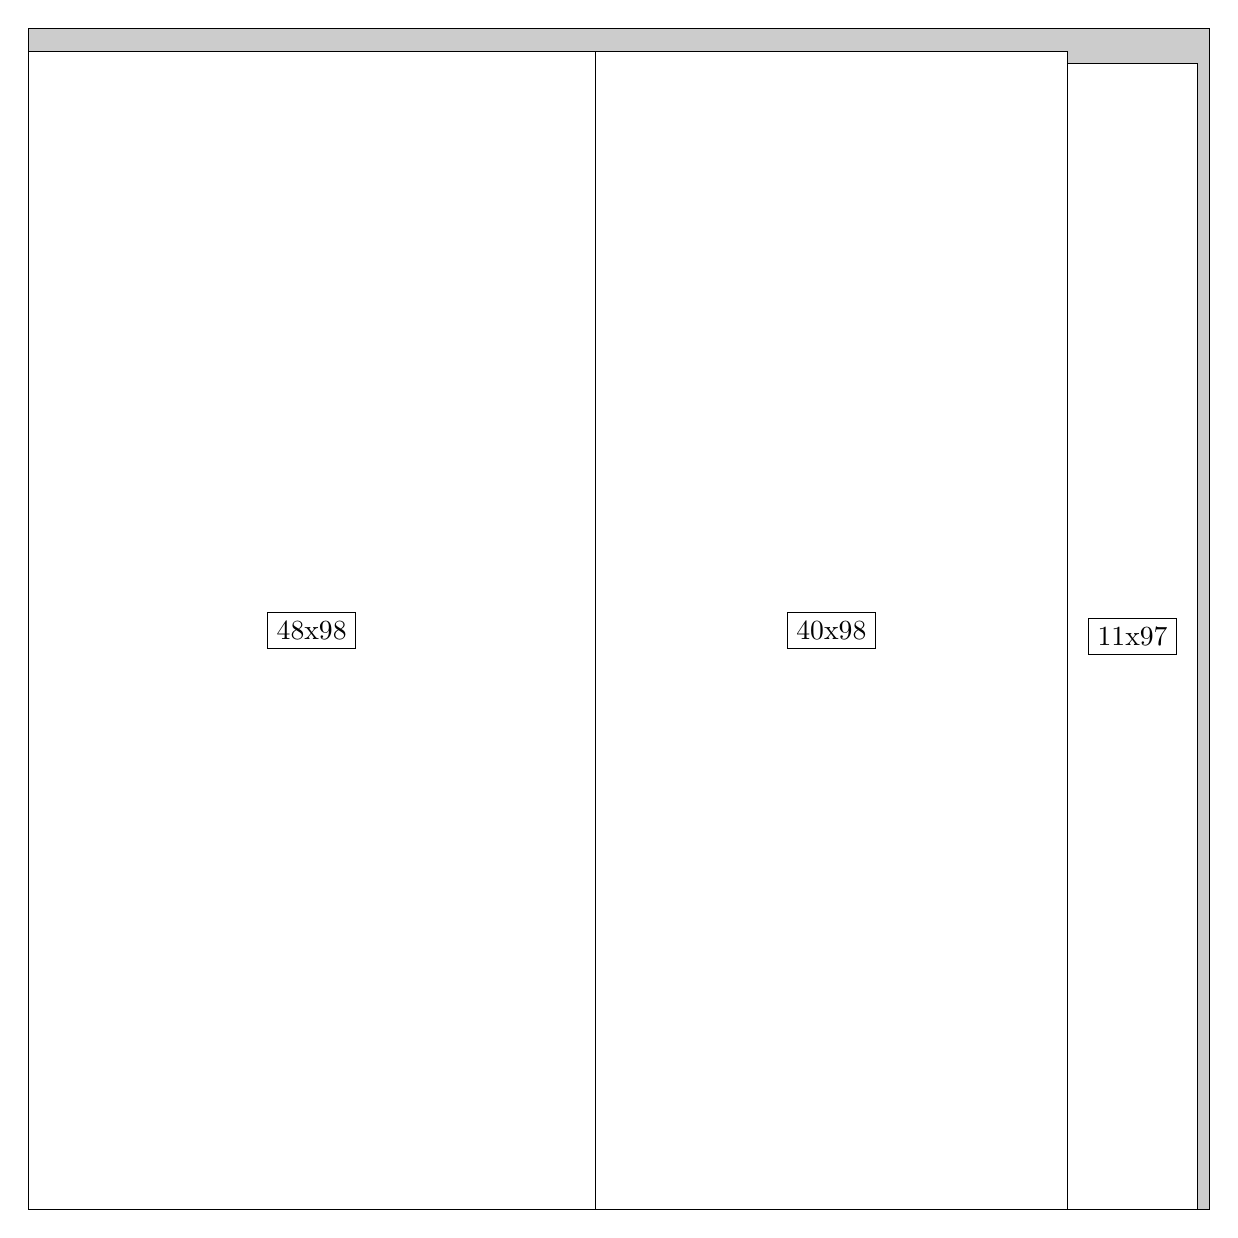
\begin{tikzpicture}[shorten >=1pt,scale=1.0,every node/.style={scale=1.0},->]
\tikzstyle{vertex}=[circle,fill=black!25,minimum size=14pt,inner sep=0pt]
\filldraw[fill=gray!40!white, draw=black] (0,0) rectangle (15.0,15.0);
\foreach \name/\x/\y/\w/\h in {48x98/0.0/0.0/7.199999999999999/14.7,40x98/7.199999999999999/0.0/6.0/14.7,11x97/13.2/0.0/1.65/14.549999999999999}
\filldraw[fill=white!40!white, draw=black] (\x,\y) rectangle node[draw] (\name) {\name} ++(\w,\h);
\end{tikzpicture}


w =48 , h =98 , x =0 , y =0 , v =4704
\par
w =40 , h =98 , x =48 , y =0 , v =3920
\par
w =11 , h =97 , x =88 , y =0 , v =1067
\par
\newpage


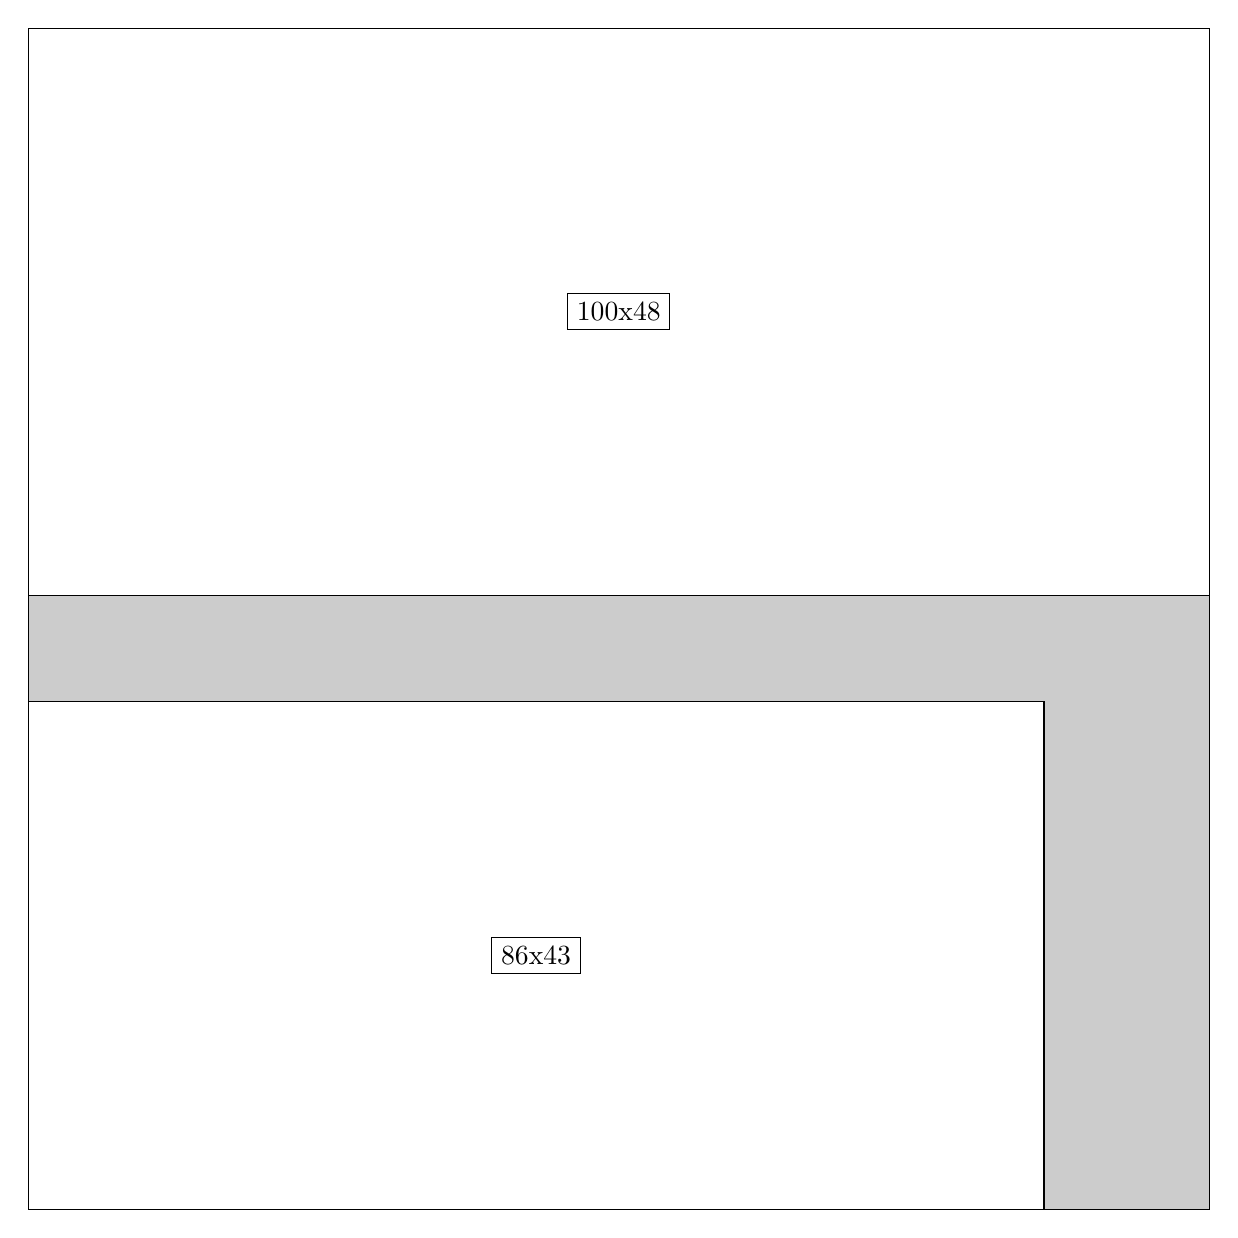
\begin{tikzpicture}[shorten >=1pt,scale=1.0,every node/.style={scale=1.0},->]
\tikzstyle{vertex}=[circle,fill=black!25,minimum size=14pt,inner sep=0pt]
\filldraw[fill=gray!40!white, draw=black] (0,0) rectangle (15.0,15.0);
\foreach \name/\x/\y/\w/\h in {100x48/0.0/7.8/15.0/7.199999999999999,86x43/0.0/0.0/12.9/6.45}
\filldraw[fill=white!40!white, draw=black] (\x,\y) rectangle node[draw] (\name) {\name} ++(\w,\h);
\end{tikzpicture}


w =100 , h =48 , x =0 , y =52 , v =4800
\par
w =86 , h =43 , x =0 , y =0 , v =3698
\par
\newpage


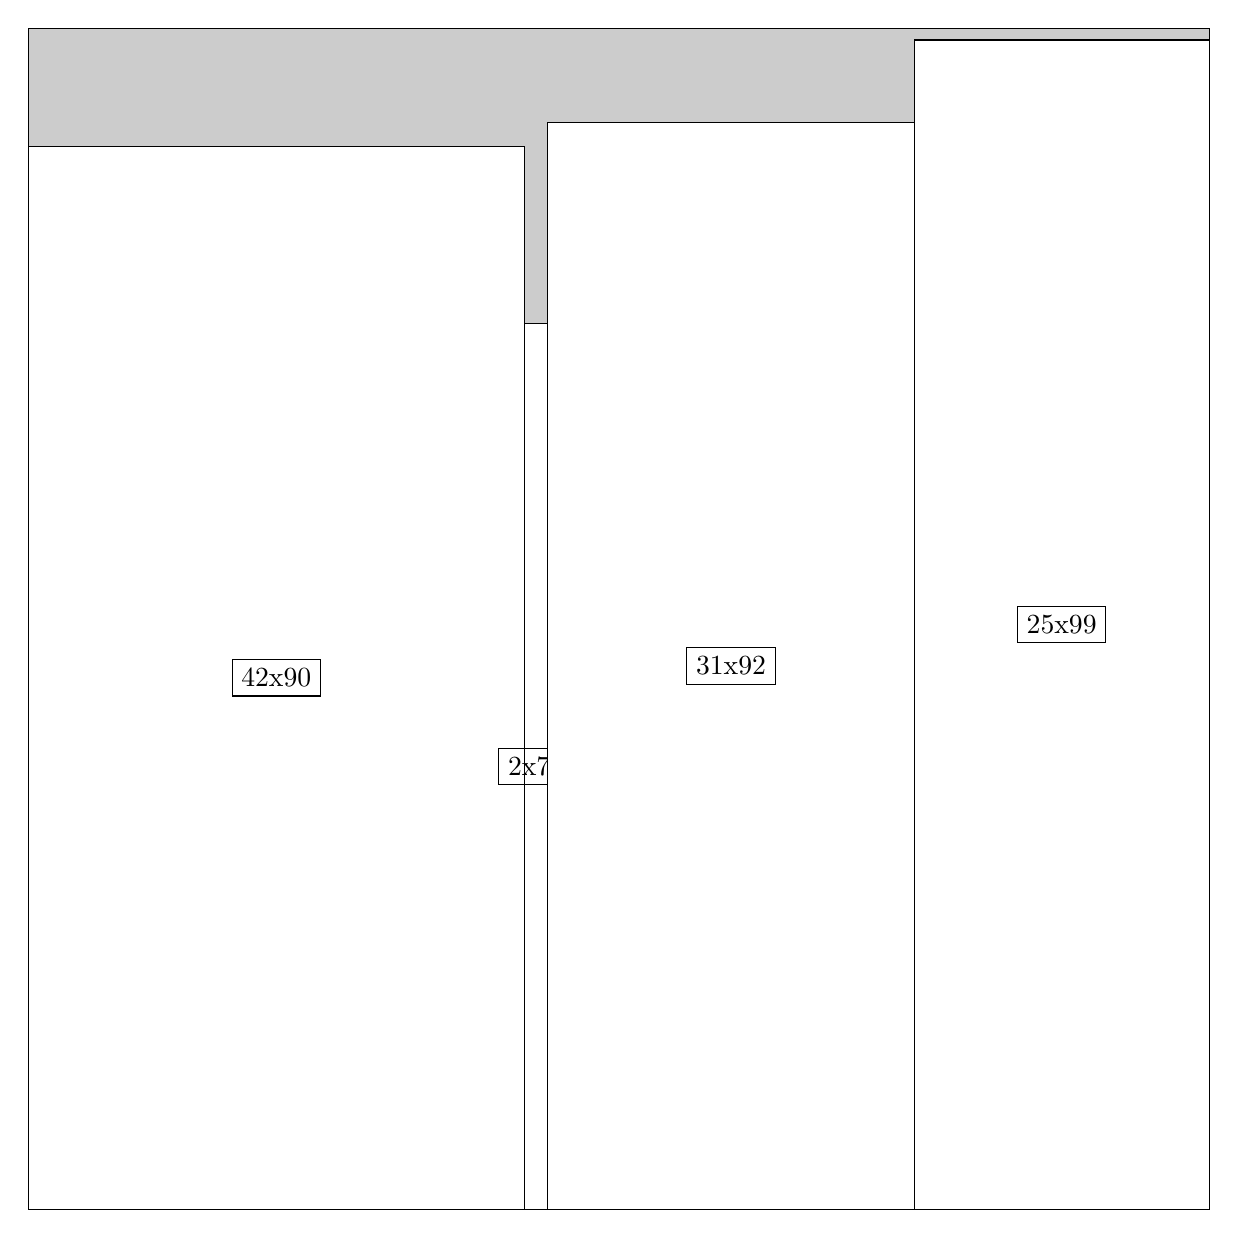
\begin{tikzpicture}[shorten >=1pt,scale=1.0,every node/.style={scale=1.0},->]
\tikzstyle{vertex}=[circle,fill=black!25,minimum size=14pt,inner sep=0pt]
\filldraw[fill=gray!40!white, draw=black] (0,0) rectangle (15.0,15.0);
\foreach \name/\x/\y/\w/\h in {42x90/0.0/0.0/6.3/13.5,2x75/6.3/0.0/0.3/11.25,31x92/6.6/0.0/4.6499999999999995/13.799999999999999,25x99/11.25/0.0/3.75/14.85}
\filldraw[fill=white!40!white, draw=black] (\x,\y) rectangle node[draw] (\name) {\name} ++(\w,\h);
\end{tikzpicture}


w =42 , h =90 , x =0 , y =0 , v =3780
\par
w =2 , h =75 , x =42 , y =0 , v =150
\par
w =31 , h =92 , x =44 , y =0 , v =2852
\par
w =25 , h =99 , x =75 , y =0 , v =2475
\par
\newpage


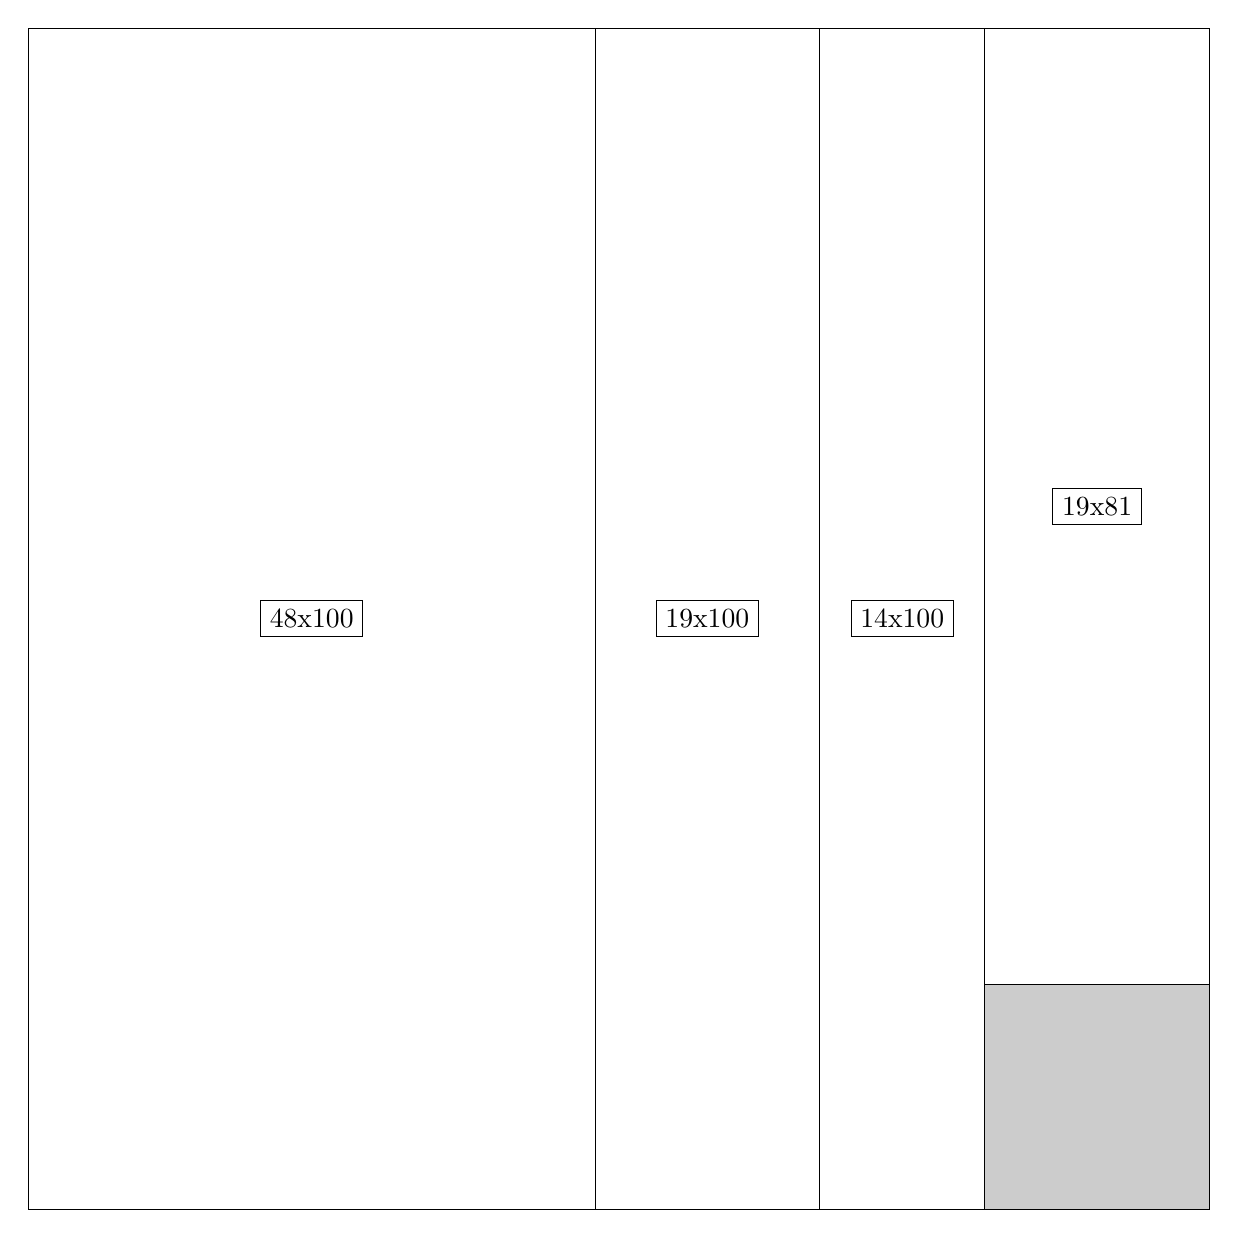
\begin{tikzpicture}[shorten >=1pt,scale=1.0,every node/.style={scale=1.0},->]
\tikzstyle{vertex}=[circle,fill=black!25,minimum size=14pt,inner sep=0pt]
\filldraw[fill=gray!40!white, draw=black] (0,0) rectangle (15.0,15.0);
\foreach \name/\x/\y/\w/\h in {48x100/0.0/0.0/7.199999999999999/15.0,19x100/7.199999999999999/0.0/2.85/15.0,19x81/12.15/2.85/2.85/12.15,14x100/10.049999999999999/0.0/2.1/15.0}
\filldraw[fill=white!40!white, draw=black] (\x,\y) rectangle node[draw] (\name) {\name} ++(\w,\h);
\end{tikzpicture}


w =48 , h =100 , x =0 , y =0 , v =4800
\par
w =19 , h =100 , x =48 , y =0 , v =1900
\par
w =19 , h =81 , x =81 , y =19 , v =1539
\par
w =14 , h =100 , x =67 , y =0 , v =1400
\par
\newpage


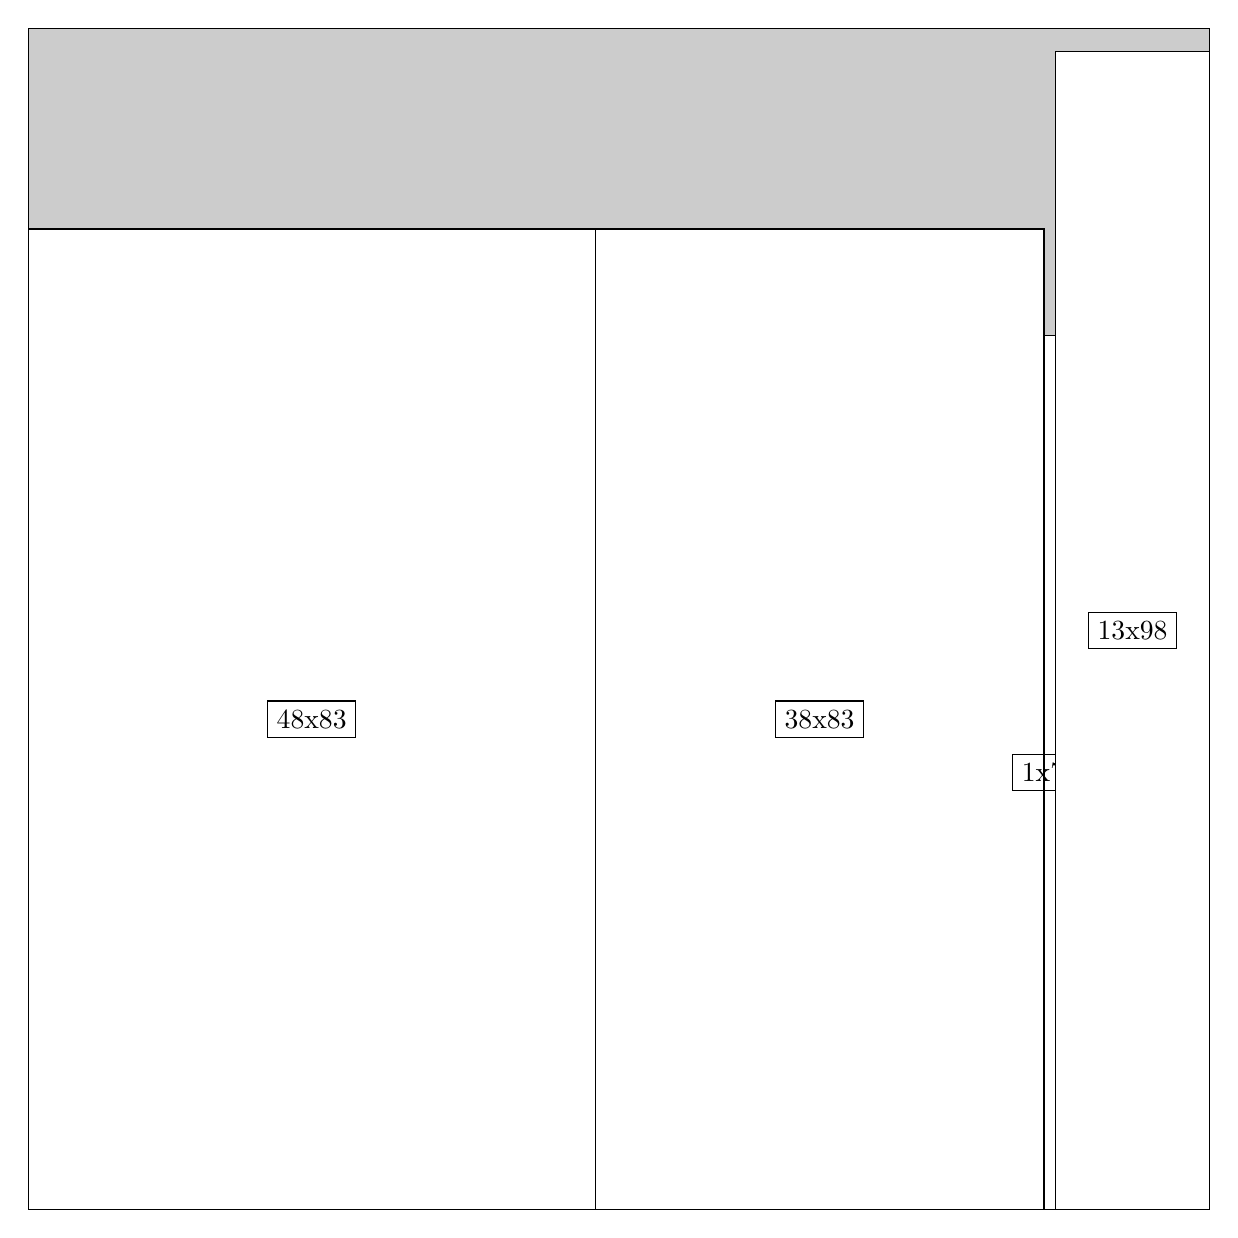
\begin{tikzpicture}[shorten >=1pt,scale=1.0,every node/.style={scale=1.0},->]
\tikzstyle{vertex}=[circle,fill=black!25,minimum size=14pt,inner sep=0pt]
\filldraw[fill=gray!40!white, draw=black] (0,0) rectangle (15.0,15.0);
\foreach \name/\x/\y/\w/\h in {48x83/0.0/0.0/7.199999999999999/12.45,38x83/7.199999999999999/0.0/5.7/12.45,1x74/12.9/0.0/0.15/11.1,13x98/13.049999999999999/0.0/1.95/14.7}
\filldraw[fill=white!40!white, draw=black] (\x,\y) rectangle node[draw] (\name) {\name} ++(\w,\h);
\end{tikzpicture}


w =48 , h =83 , x =0 , y =0 , v =3984
\par
w =38 , h =83 , x =48 , y =0 , v =3154
\par
w =1 , h =74 , x =86 , y =0 , v =74
\par
w =13 , h =98 , x =87 , y =0 , v =1274
\par
\newpage


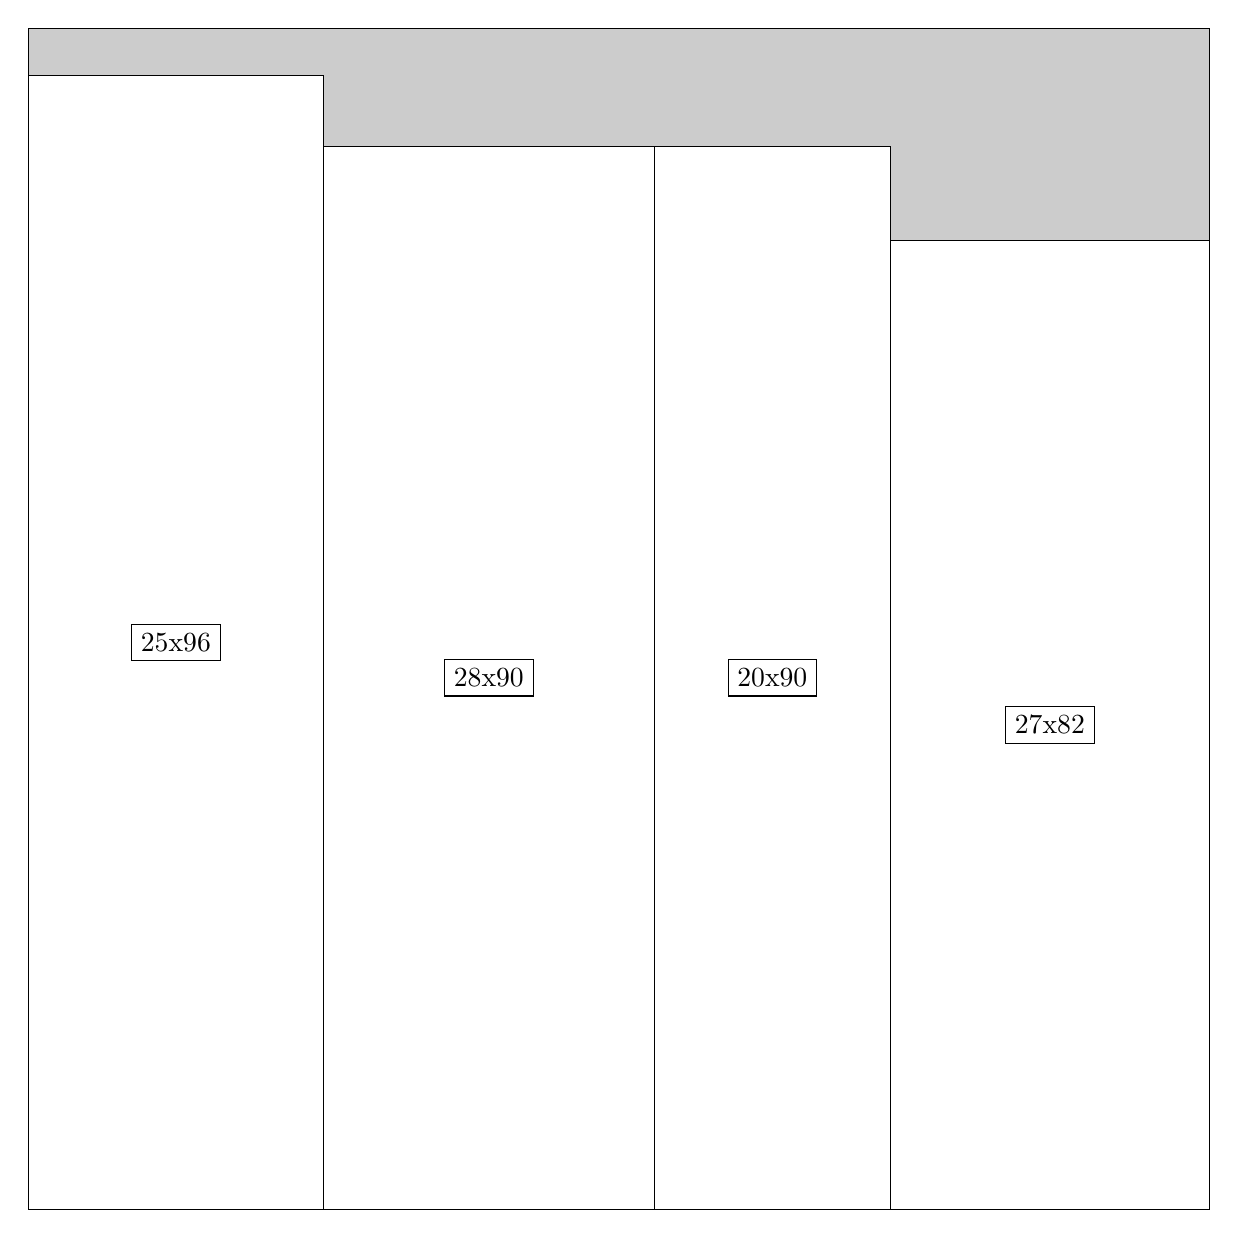
\begin{tikzpicture}[shorten >=1pt,scale=1.0,every node/.style={scale=1.0},->]
\tikzstyle{vertex}=[circle,fill=black!25,minimum size=14pt,inner sep=0pt]
\filldraw[fill=gray!40!white, draw=black] (0,0) rectangle (15.0,15.0);
\foreach \name/\x/\y/\w/\h in {28x90/3.75/0.0/4.2/13.5,25x96/0.0/0.0/3.75/14.399999999999999,27x82/10.95/0.0/4.05/12.299999999999999,20x90/7.949999999999999/0.0/3.0/13.5}
\filldraw[fill=white!40!white, draw=black] (\x,\y) rectangle node[draw] (\name) {\name} ++(\w,\h);
\end{tikzpicture}


w =28 , h =90 , x =25 , y =0 , v =2520
\par
w =25 , h =96 , x =0 , y =0 , v =2400
\par
w =27 , h =82 , x =73 , y =0 , v =2214
\par
w =20 , h =90 , x =53 , y =0 , v =1800
\par
\newpage


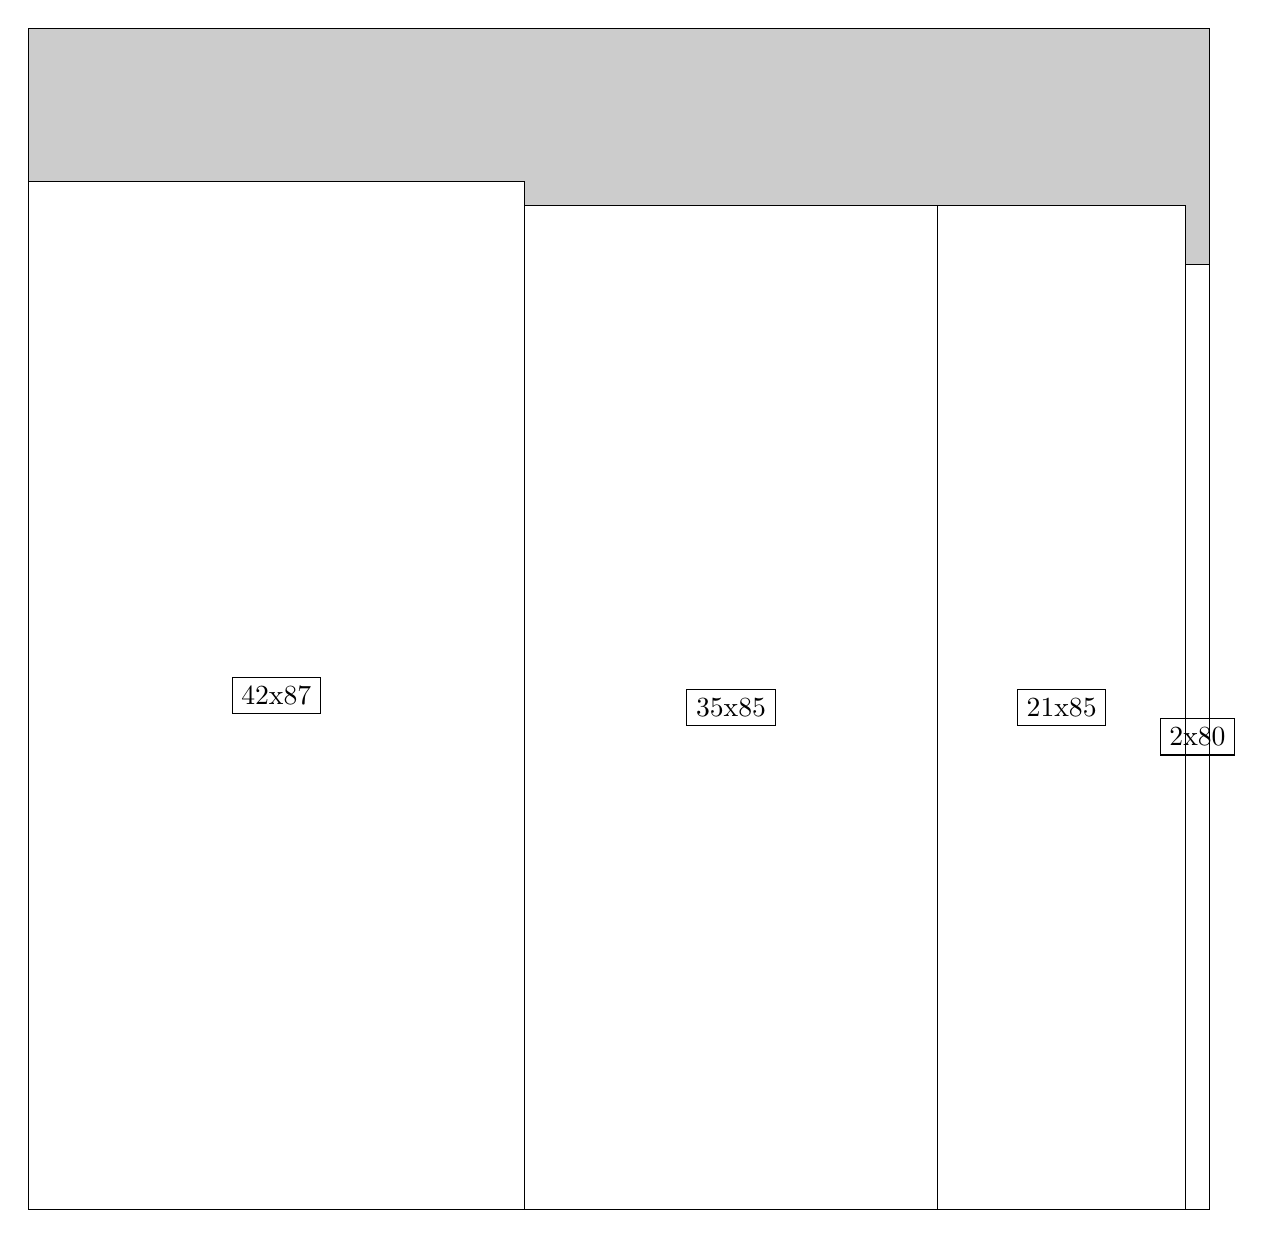
\begin{tikzpicture}[shorten >=1pt,scale=1.0,every node/.style={scale=1.0},->]
\tikzstyle{vertex}=[circle,fill=black!25,minimum size=14pt,inner sep=0pt]
\filldraw[fill=gray!40!white, draw=black] (0,0) rectangle (15.0,15.0);
\foreach \name/\x/\y/\w/\h in {42x87/0.0/0.0/6.3/13.049999999999999,35x85/6.3/0.0/5.25/12.75,21x85/11.549999999999999/0.0/3.15/12.75,2x80/14.7/0.0/0.3/12.0}
\filldraw[fill=white!40!white, draw=black] (\x,\y) rectangle node[draw] (\name) {\name} ++(\w,\h);
\end{tikzpicture}


w =42 , h =87 , x =0 , y =0 , v =3654
\par
w =35 , h =85 , x =42 , y =0 , v =2975
\par
w =21 , h =85 , x =77 , y =0 , v =1785
\par
w =2 , h =80 , x =98 , y =0 , v =160
\par
\newpage


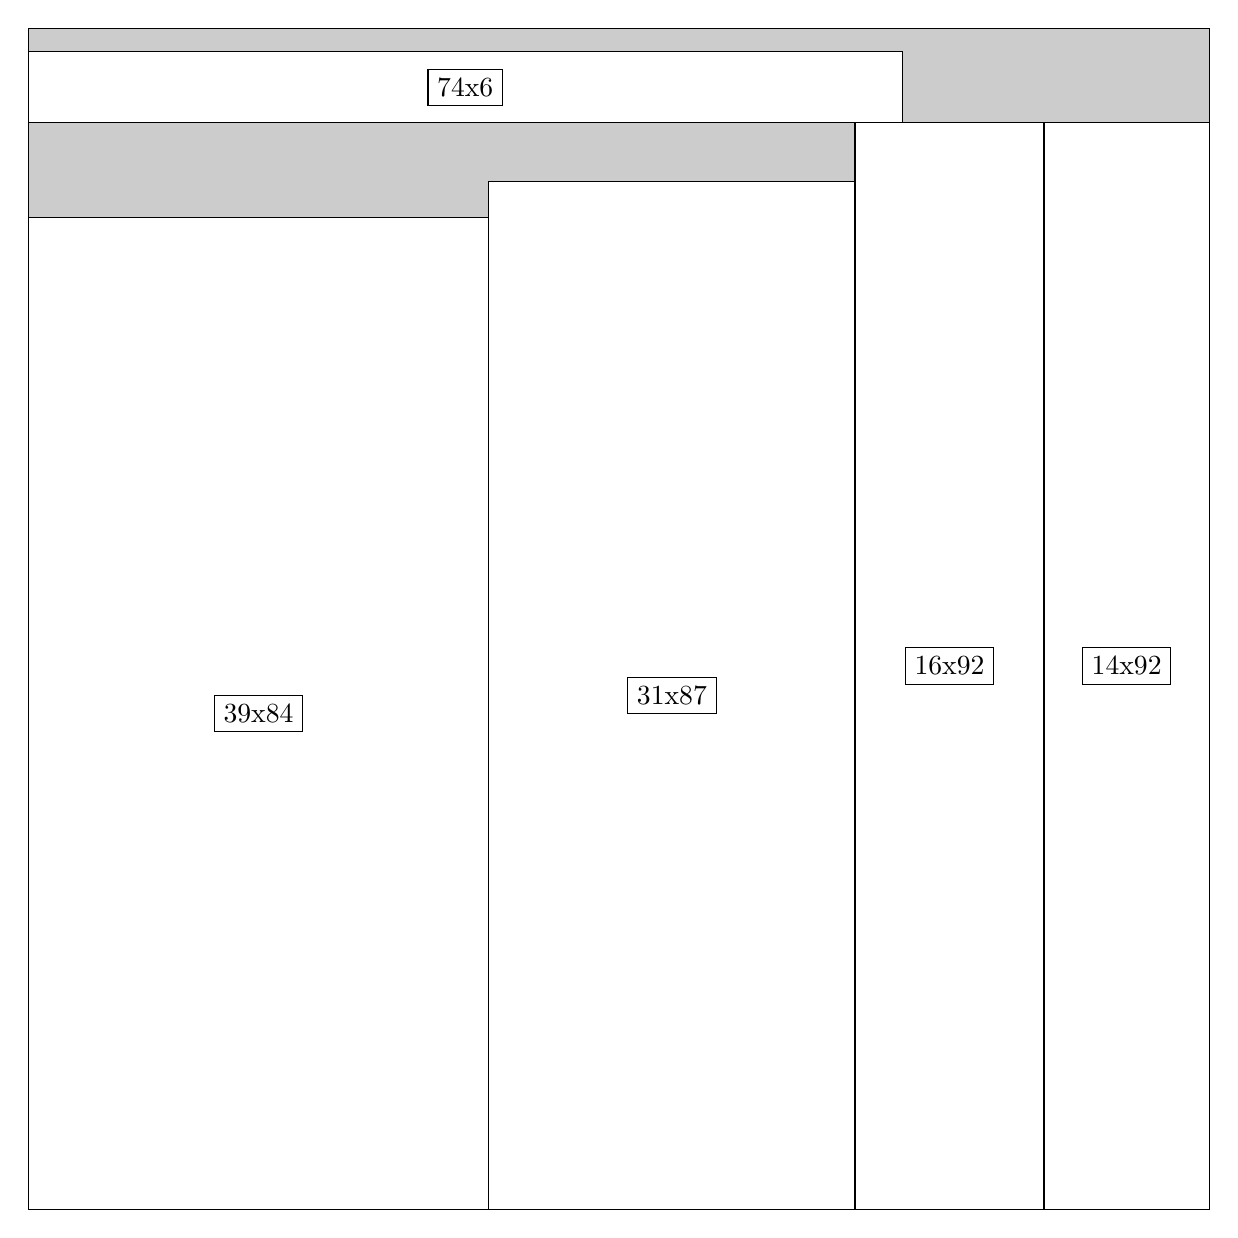
\begin{tikzpicture}[shorten >=1pt,scale=1.0,every node/.style={scale=1.0},->]
\tikzstyle{vertex}=[circle,fill=black!25,minimum size=14pt,inner sep=0pt]
\filldraw[fill=gray!40!white, draw=black] (0,0) rectangle (15.0,15.0);
\foreach \name/\x/\y/\w/\h in {39x84/0.0/0.0/5.85/12.6,31x87/5.85/0.0/4.6499999999999995/13.049999999999999,16x92/10.5/0.0/2.4/13.799999999999999,14x92/12.9/0.0/2.1/13.799999999999999,74x6/0.0/13.799999999999999/11.1/0.8999999999999999}
\filldraw[fill=white!40!white, draw=black] (\x,\y) rectangle node[draw] (\name) {\name} ++(\w,\h);
\end{tikzpicture}


w =39 , h =84 , x =0 , y =0 , v =3276
\par
w =31 , h =87 , x =39 , y =0 , v =2697
\par
w =16 , h =92 , x =70 , y =0 , v =1472
\par
w =14 , h =92 , x =86 , y =0 , v =1288
\par
w =74 , h =6 , x =0 , y =92 , v =444
\par
\newpage


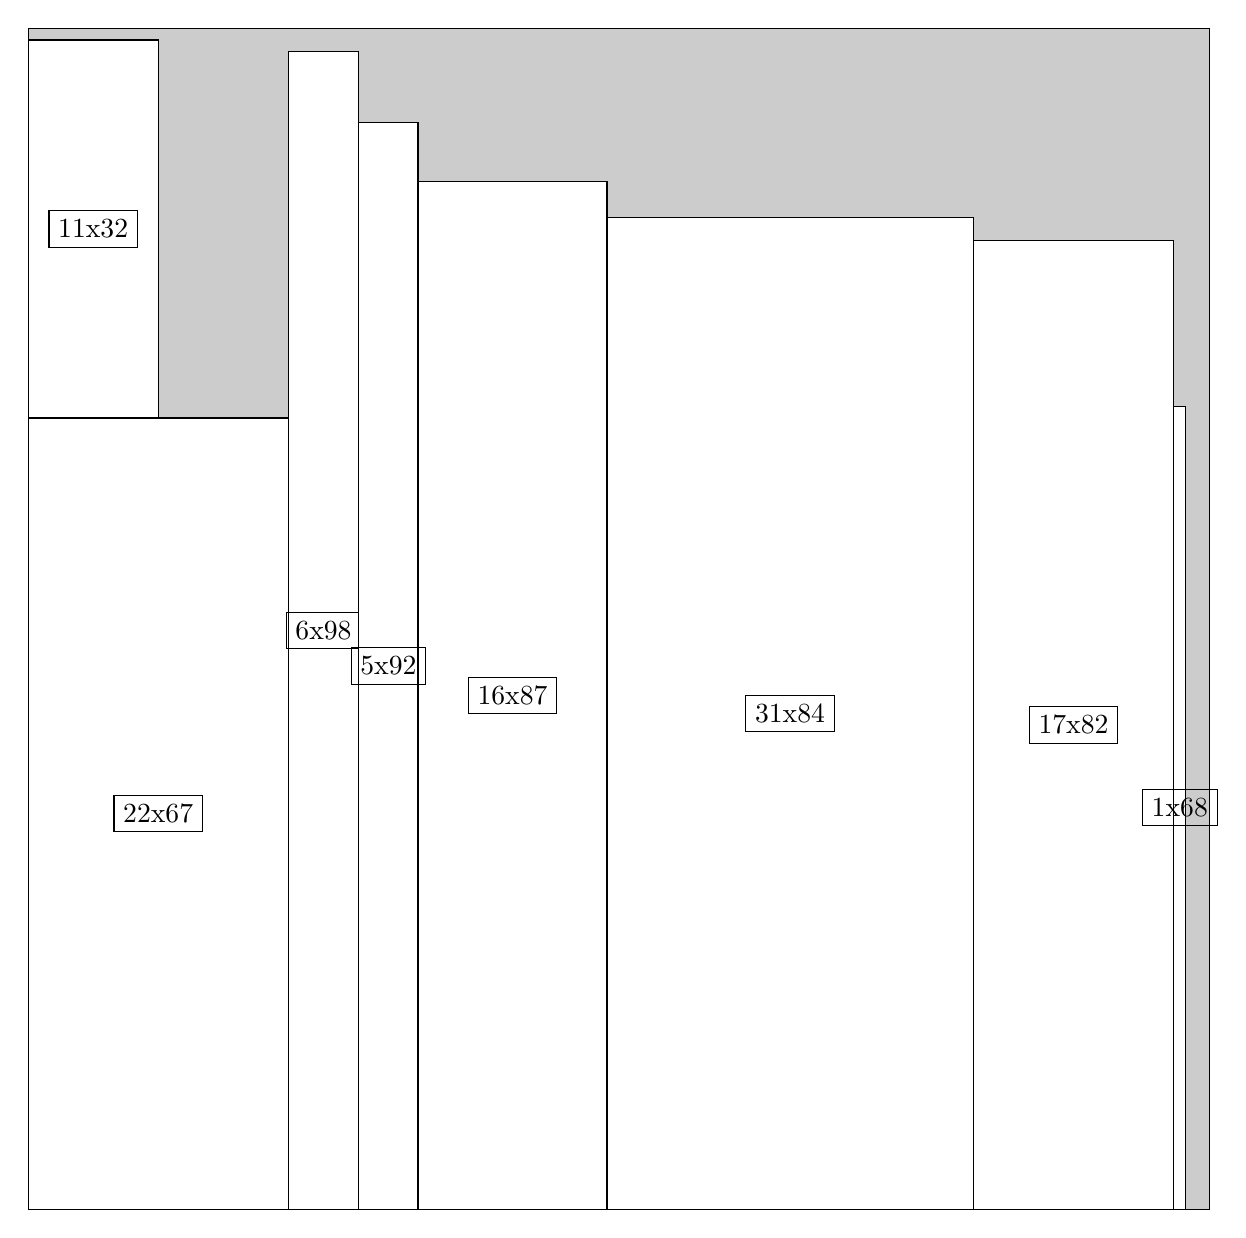
\begin{tikzpicture}[shorten >=1pt,scale=1.0,every node/.style={scale=1.0},->]
\tikzstyle{vertex}=[circle,fill=black!25,minimum size=14pt,inner sep=0pt]
\filldraw[fill=gray!40!white, draw=black] (0,0) rectangle (15.0,15.0);
\foreach \name/\x/\y/\w/\h in {31x84/7.35/0.0/4.6499999999999995/12.6,16x87/4.95/0.0/2.4/13.049999999999999,22x67/0.0/0.0/3.3/10.049999999999999,17x82/12.0/0.0/2.55/12.299999999999999,6x98/3.3/0.0/0.8999999999999999/14.7,5x92/4.2/0.0/0.75/13.799999999999999,11x32/0.0/10.049999999999999/1.65/4.8,1x68/14.549999999999999/0.0/0.15/10.2}
\filldraw[fill=white!40!white, draw=black] (\x,\y) rectangle node[draw] (\name) {\name} ++(\w,\h);
\end{tikzpicture}


w =31 , h =84 , x =49 , y =0 , v =2604
\par
w =16 , h =87 , x =33 , y =0 , v =1392
\par
w =22 , h =67 , x =0 , y =0 , v =1474
\par
w =17 , h =82 , x =80 , y =0 , v =1394
\par
w =6 , h =98 , x =22 , y =0 , v =588
\par
w =5 , h =92 , x =28 , y =0 , v =460
\par
w =11 , h =32 , x =0 , y =67 , v =352
\par
w =1 , h =68 , x =97 , y =0 , v =68
\par
\newpage


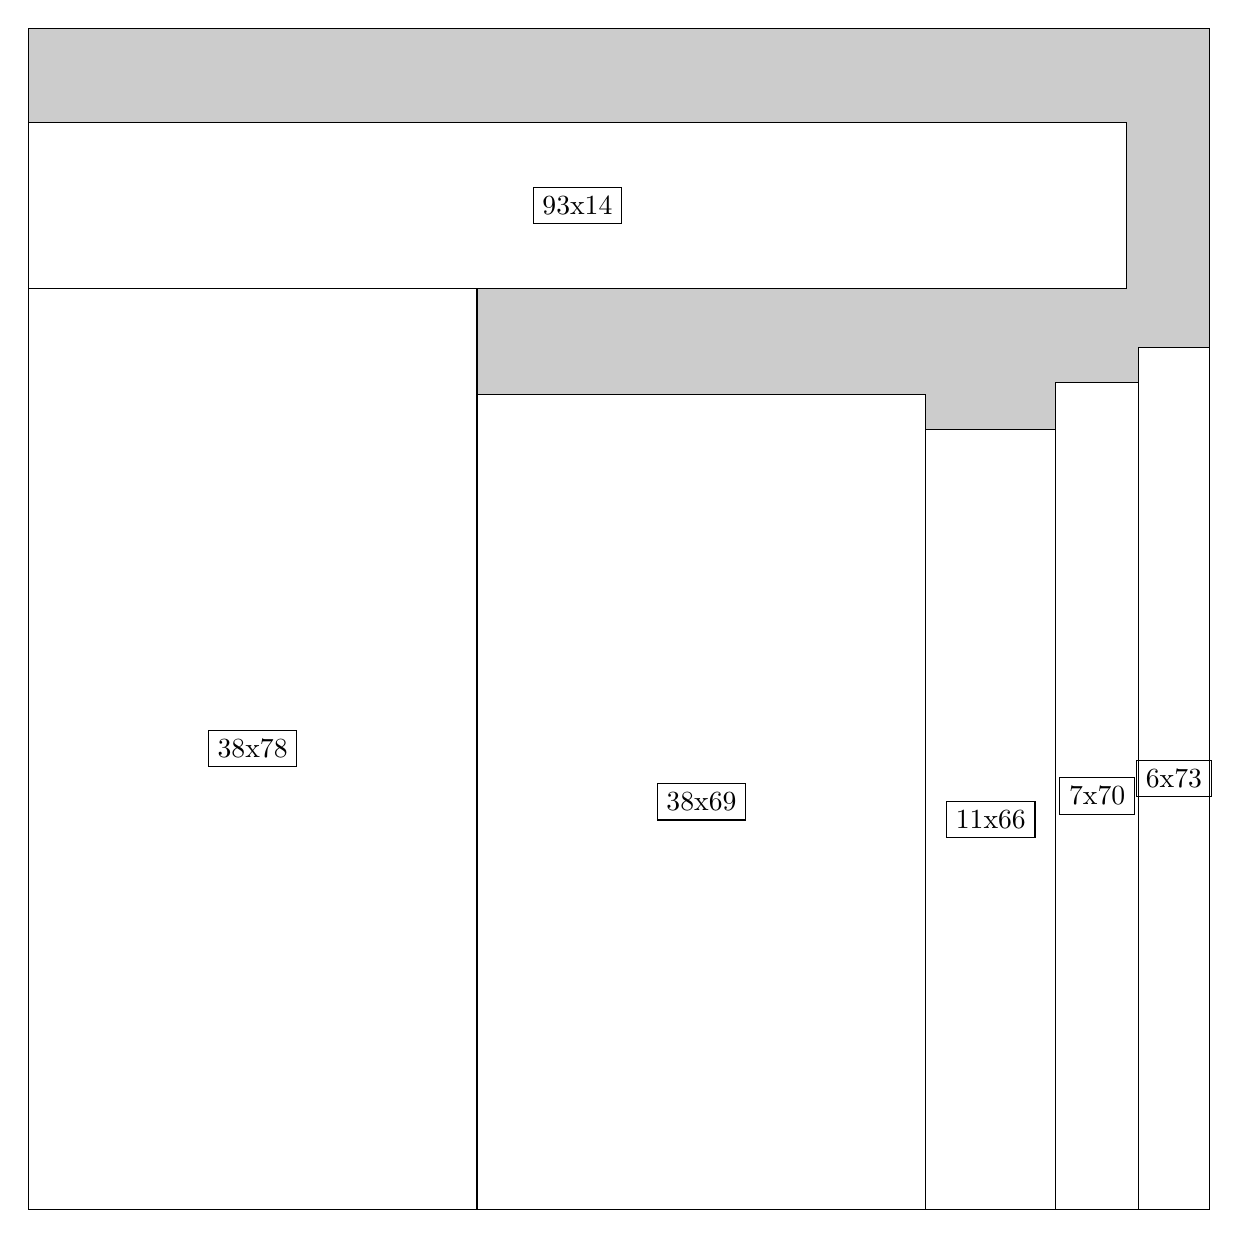
\begin{tikzpicture}[shorten >=1pt,scale=1.0,every node/.style={scale=1.0},->]
\tikzstyle{vertex}=[circle,fill=black!25,minimum size=14pt,inner sep=0pt]
\filldraw[fill=gray!40!white, draw=black] (0,0) rectangle (15.0,15.0);
\foreach \name/\x/\y/\w/\h in {38x78/0.0/0.0/5.7/11.7,38x69/5.7/0.0/5.7/10.35,93x14/0.0/11.7/13.95/2.1,11x66/11.4/0.0/1.65/9.9,7x70/13.049999999999999/0.0/1.05/10.5,6x73/14.1/0.0/0.8999999999999999/10.95}
\filldraw[fill=white!40!white, draw=black] (\x,\y) rectangle node[draw] (\name) {\name} ++(\w,\h);
\end{tikzpicture}


w =38 , h =78 , x =0 , y =0 , v =2964
\par
w =38 , h =69 , x =38 , y =0 , v =2622
\par
w =93 , h =14 , x =0 , y =78 , v =1302
\par
w =11 , h =66 , x =76 , y =0 , v =726
\par
w =7 , h =70 , x =87 , y =0 , v =490
\par
w =6 , h =73 , x =94 , y =0 , v =438
\par
\newpage


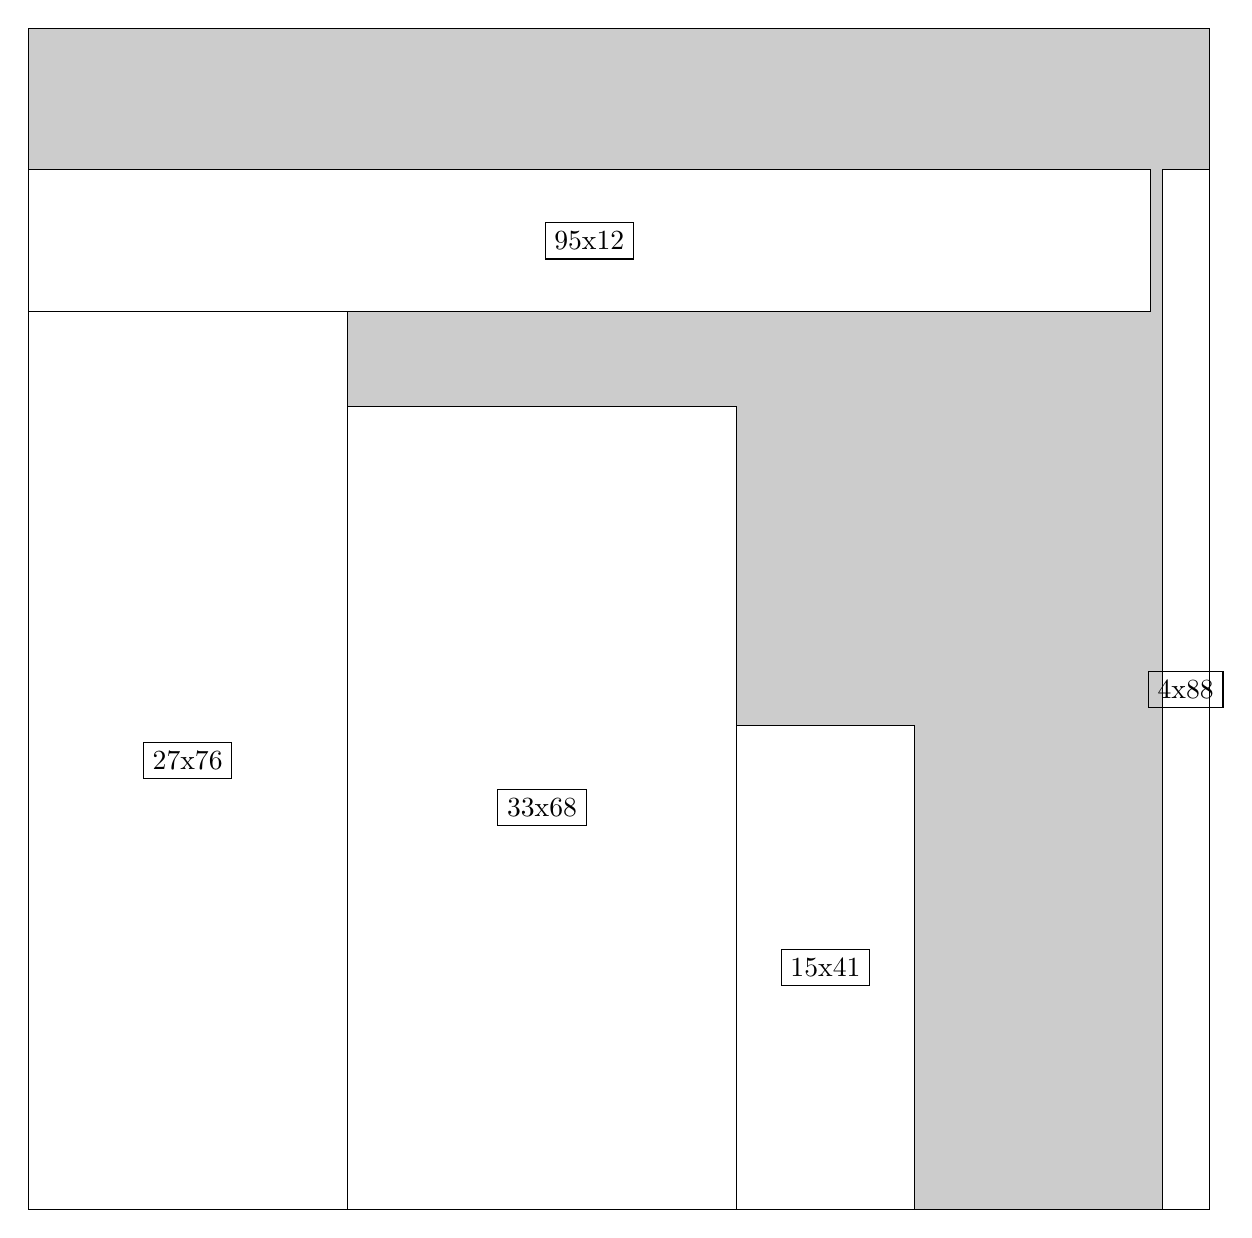
\begin{tikzpicture}[shorten >=1pt,scale=1.0,every node/.style={scale=1.0},->]
\tikzstyle{vertex}=[circle,fill=black!25,minimum size=14pt,inner sep=0pt]
\filldraw[fill=gray!40!white, draw=black] (0,0) rectangle (15.0,15.0);
\foreach \name/\x/\y/\w/\h in {27x76/0.0/0.0/4.05/11.4,33x68/4.05/0.0/4.95/10.2,95x12/0.0/11.4/14.25/1.7999999999999998,15x41/9.0/0.0/2.25/6.1499999999999995,4x88/14.399999999999999/0.0/0.6/13.2}
\filldraw[fill=white!40!white, draw=black] (\x,\y) rectangle node[draw] (\name) {\name} ++(\w,\h);
\end{tikzpicture}


w =27 , h =76 , x =0 , y =0 , v =2052
\par
w =33 , h =68 , x =27 , y =0 , v =2244
\par
w =95 , h =12 , x =0 , y =76 , v =1140
\par
w =15 , h =41 , x =60 , y =0 , v =615
\par
w =4 , h =88 , x =96 , y =0 , v =352
\par
\newpage


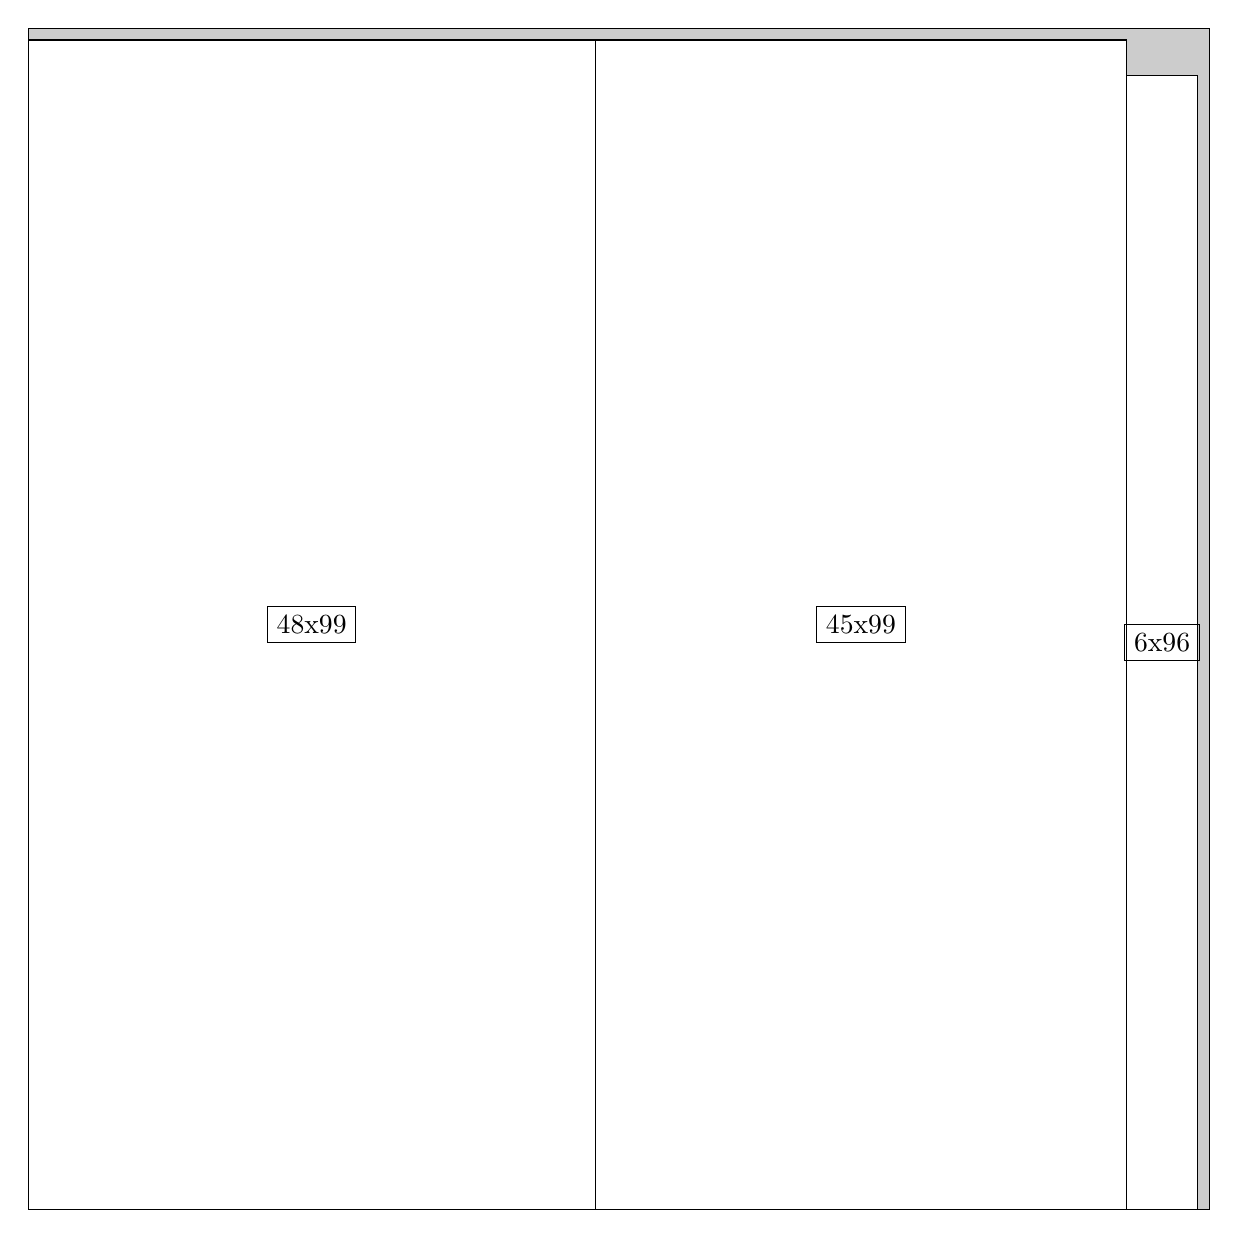
\begin{tikzpicture}[shorten >=1pt,scale=1.0,every node/.style={scale=1.0},->]
\tikzstyle{vertex}=[circle,fill=black!25,minimum size=14pt,inner sep=0pt]
\filldraw[fill=gray!40!white, draw=black] (0,0) rectangle (15.0,15.0);
\foreach \name/\x/\y/\w/\h in {48x99/0.0/0.0/7.199999999999999/14.85,45x99/7.199999999999999/0.0/6.75/14.85,6x96/13.95/0.0/0.8999999999999999/14.399999999999999}
\filldraw[fill=white!40!white, draw=black] (\x,\y) rectangle node[draw] (\name) {\name} ++(\w,\h);
\end{tikzpicture}


w =48 , h =99 , x =0 , y =0 , v =4752
\par
w =45 , h =99 , x =48 , y =0 , v =4455
\par
w =6 , h =96 , x =93 , y =0 , v =576
\par
\newpage


\end{document}